\chapter {Arduino Web Version}

\section{Introduction}


The Arduino Web Editor allows you to write code and upload sketches to any official Arduino board directly from your web browser (Chrome, Firefox, Safari and Edge). \cite{arduinoWebEditor:2024}

This IDE (Integrated Development Environment) is part of Arduino Create, an online platform that enables developers to write code, access tutorials, configure boards, and share projects. Designed to provide users with a continuous workflow, Arduino Create connects the dots between each part of a developer's journey from inspiration to implementation. Meaning, you now have the ability to manage every aspect of your project right from a single dashboard.

The Arduino Web Editor is hosted online, therefore it is always be up-to-date with the latest features and support for new boards.This IDE lets you write code and save it to the Cloud, always backing it up and making it accessible from any device. It automatically recognizes any Arduino board connected to your PC, and configures itself accordingly.

All you need to get started is an Arduino account. The following steps can guide you to start using the Arduino Web Editor: \cite{arduinoWebEditor:2024}

\subsection{Using the online IDE}
After logging in, you are ready to start using the Arduino Web Editor. The web app is divided into three main columns. ~\ref{web-editor}

\begin{figure}
	\begin{center}
		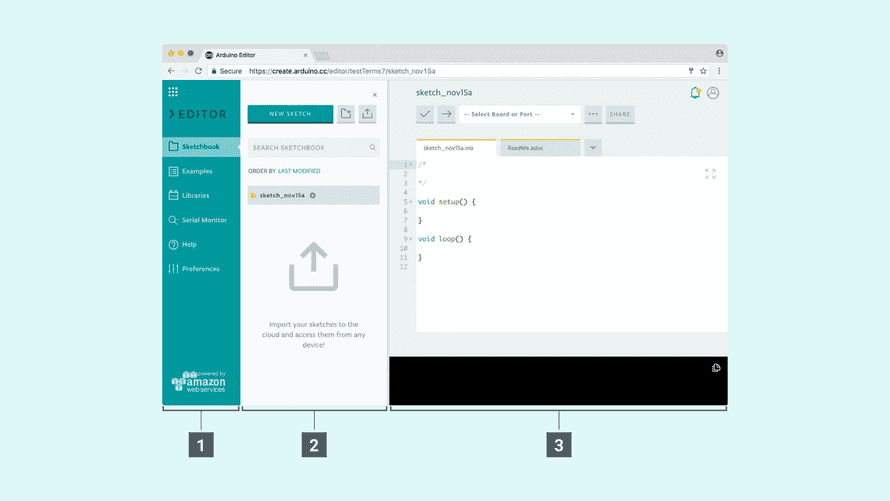
\includegraphics[width=0.7\linewidth]{Images/Arduino/web-editor.png}
		\caption{web-editor}
		\label{web-editor}
	\end{center}
\end{figure}
The Arduino Web Editor’s interface is as follows: 
\begin{enumerate}
	\item The first column lets you navigate between:
	\begin{itemize}
		\item \textbf{Your Sketchbook}: a collection of all your sketches (a sketch is a program you upload on your board).
		\item \textbf{Examples}: read-only sketches that demonstrate all the basic Arduino commands (built-in tab), and the behavior of your libraries (from the libraries tab).
		\item \textbf{Libraries}: packages that can be included to your sketch to provide extra functionalities.
		\item \textbf{Serial monitor}: a feature that enables you to monitor, receive and send data to and from your board via the USB cable.
		\item \textbf{Help}: helpful links and a glossary about Arduino terms.
		\item \textbf{Preferences}: options to customize the look and behavior of your editor, such as text size and color theme.		
	\end{itemize}
	\item The second column views the content of the chosen option.
	\item The third column, the code area, is the one you will use the most. Here, you can write code, verify it and upload it to your boards, save your sketches on the Cloud, and share them with anyone you want.
\end{enumerate}

Now that we are all set up, let’s try to make the board blink!

\begin{enumerate}
	\item Connect your Arduino or Genuino board to your computer. Boards and serial ports are auto-discovered and selectable in a single dropdown. Pick the Arduino/Genuino board you want to upload to from the list at the top of the third column.\cite{arduinoWebEditor:2024}
	\item Let’s try with an example: Choose Examples on the menu on the left (first column), then Basic and Blink. The Blink sketch is now displayed in the code area. 
	\item To upload it to your board, press the "Upload" button near the dropdown menu. While the code is verifying and uploading, a "BUSY" label replaces the upload button. If the upload is successful, the message "Success: done uploading" will appear in the bottom output area.
	\item Once the upload is complete, you should see on your board the yellow LED with an L next to it start blinking. You can adjust the speed of blinking by changing the delay number in the parenthesis to 100, and upload the Blink sketch again. Now the LED should blink much faster ~\ref{finding-an-example}.
\end{enumerate}

\begin{figure}
	\begin{center}
		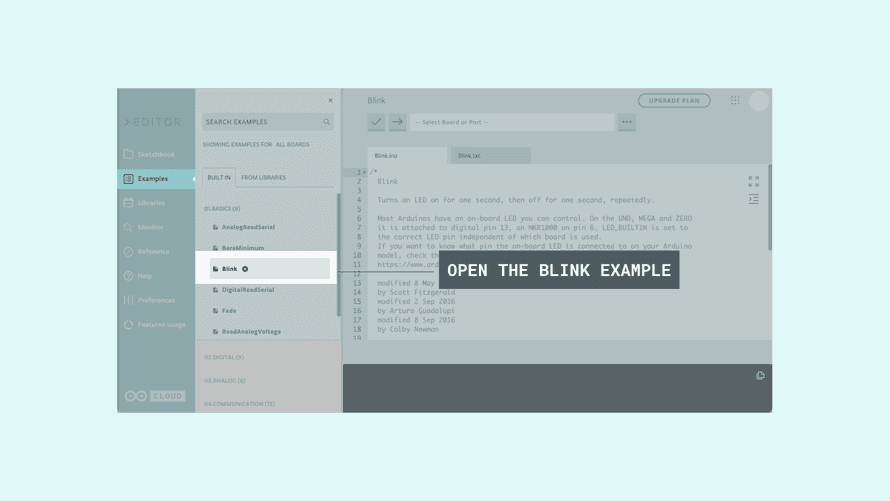
\includegraphics[width=0.7\linewidth]{Images/Arduino/finding-an-example.png}
		\caption{finding-an-example}
		\label{finding-an-example}
	\end{center}
\end{figure} 

\section{Arduino Libraries}
The process of setting up libraries on the online IDE (Arduino Cloud Editor) is quite similar to the offline one: \cite{arduinoLibraries:2025} \cite{arduinoCloud:2025}

\begin{enumerate}
	\item Login to the Arduino Cloud.
	\item Create or open a sketch.
	\item Open the "Libraries" tab from the left menu, and search for libraries. The list displays read-only libraries, authored and maintained by the Arduino team and its partners.
	\item When you find the library, you can add it to your sketch by selecting the "Include" button. You can also see the related examples, and select a specific version, if available.
	\item If you can't find a specific library on the list, you can search every existing library through the search bar. You also have the option to add them to your favorites list by clicking on the star next to the library you want. Once you star a library, you can view it under the "favorites" tab and use its examples (if available).
\end{enumerate} 

\section{Data Security}
\begin{itemize}
	\item \textbf{Encryption}: The web version of Arduino IDE should use strong encryption protocols to secure data transmitted between the user's browser and the server, preventing unauthorized access.
	\item \textbf{Secure Storage}: User data, including login credentials and project files, should be encrypted at rest to protect against unauthorized access or tampering.
\end{itemize}

\subsection{Authentication and Authorization}
\begin{itemize}
	\item \textbf{Strong Password Policies}: Enforce password complexity and offer multi-factor authentication to enhance account security.
	\item \textbf{Role-Based Access Control}: Implement role-based access to ensure users only access necessary resources, preventing unauthorized access to sensitive data.
\end{itemize}

\subsection{Secure Code Execution}
\begin{itemize}
	\item \textbf{Sandboxing}: Execute user-uploaded code in a sandboxed environment to restrict access to system resources and prevent malicious actions.
	\item \textbf{Code Validation}: Validate user code to detect and prevent vulnerabilities like code injection or buffer overflows before execution.
\end{itemize}

\subsection{Protection Against Malware}
\begin{itemize}
	\item \textbf{Code Scanning}: Use code scanning to detect and block malicious code by analyzing for malware signatures or suspicious patterns.
	\item \textbf{Antivirus Integration}: Integrate antivirus solutions to scan uploaded files for viruses or malicious content before execution.
\end{itemize}

\subsection{Privacy Policies}
\begin{itemize}
	\item \textbf{Transparency}: Maintain clear privacy policies outlining data collection, storage, usage, retention periods, and third-party sharing practices.
	\item \textbf{User Consent}: Inform users about privacy practices and obtain explicit consent for data processing, allowing them to review and modify privacy settings.
\end{itemize}

\subsection{Regular Updates and Maintenance}
\begin{itemize}
	\item \textbf{Patch Management}: Regularly update software components, libraries, and dependencies to address security vulnerabilities promptly.
	\item \textbf{Security Audits}: Conduct regular security audits and penetration testing to identify and remediate potential weaknesses.
\end{itemize}

\subsection{User Awareness}
\begin{itemize}
	\item \textbf{Security Education}: Provide resources on secure coding practices to help users avoid vulnerabilities like XSS, SQL injection, and insecure object references.
	\item \textbf{Security Alerts}: Notify users about security-related issues, such as suspicious login attempts or unauthorized access.
\end{itemize}





